\documentclass[english]{article}

\usepackage[a4paper,margin=2cm]{geometry}
\usepackage{setspace}
\onehalfspacing

\usepackage{amsmath}
\usepackage{amsthm}
\usepackage{amssymb}

\usepackage{babel}

\usepackage{mathptmx}
\usepackage{amsmath}
\usepackage{graphicx}
\usepackage{color}

\newcommand{\Tr}{{\bf Tr}}
\newcommand{\R}{\mathbb{R}}
\newcommand{\E}{\mathbb{E}}
\newcommand{\N}{\mathcal{N}}
%\newcommand{\Pr}{ \text{Pr} }


\newtheorem{theorem}{Theorem}[section]
\newtheorem{conject}{Conjecture}[section]

\newtheorem{lemma}{Lemma}[section]
\newtheorem{corollary}{Corollary}[section]
\newtheorem{proposition}{Proposition}[section]


%% Choose one of the following (if not choosing the  
%% default, viz., Computer Modern, font family):
 %\usepackage{lmodern}
 %%
 %\usepackage{mathpazo}
% \usepackage[theoremfont]{newpxmath} \usepackage{newpxmath}
 %\usepackage{kpfonts}
 %%
 %\usepackage{mathptmx}
 %\usepackage{times,mtpro2}
 %\usepackage{stix}
 %\usepackage{txfonts}
 %\usepackage{newtxtext,newtxmath}
 %%
 
 %\usepackage{libertine} \usepackage[libertine]{newtxmath}
 
 %\usepackage{newpxtext} \usepackage[euler-digits]{eulervm}


\begin{document}


\title{Math 690 F2017: Topics in Data Analysis and Computation\\
Homework 3}

\author{Xiuyuan Cheng}

\date{}

\maketitle


This problem set asks to compare (a) Isomap, (b)LLE, 
(c) Laplacian eigenmap,
and (d) t-SNE 
to synthetic manifold data and handwritten digits data.

\begin{enumerate}

\item
Generate data by uniformly sampling $n=1000$ points on a closed curve embedded in $\R^3$, e.g.
\[
(\cos(2\pi t), \sin(2\pi t), \cos(8\pi t))^T,
\quad 0 \le t \le 1.
\]
A typical output is shown in Figure below. 

\begin{figure}[h]
\centering{
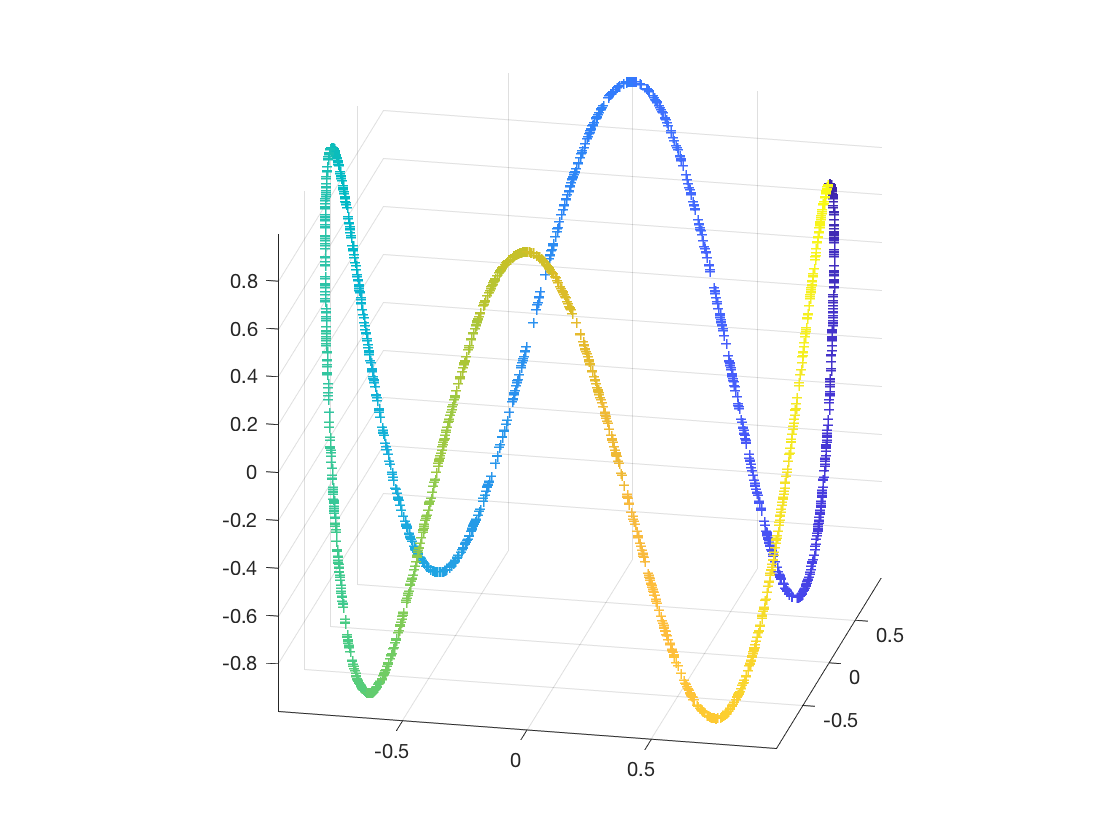
\includegraphics[width=0.6\linewidth]{curve1.png}
}
\caption{
Manifold data, no noise.
}
\label{fig:1}
\end{figure}

(1) 
Effect of $n$:
what are the embedding like for the (a)-(d) methods? What the effect of having $n$ increased e.g. doubled?


(2) 
Effect of parameter:
in (a)-(c), what is the effect of choosing different $k$ in constructing the kNN-graph? 
Similarly, what is the effect of choosing different $\epsilon$ in constructing the $\epsilon$-graph in (a),(c)?
For (d), the corresponding parameter of $k$ is the ``perplexity".

(3) 
Effect of noise:
what if add Gaussian noise ${\cal N}(0, \sigma^2 I_3)$ to the data? What is the influence of the noise level $\sigma$? 

(4)
Effect of ambient dimension:
what if the curve is embedded in higher dimension than 3, e.g. in dimension 10 or 30? How does Gaussian noise change the embedding?

(5)
Effect of topology:
what if changing the curve into a belt (intrinsic dimension 2)? How does the width of the belt affect the embeddings?
Question(*): What happens if it is a Mobius belt?

\item
Load the handwritten digits for example MNIST and repeat (1)-(3) of Problem 1. To simplify visualization, you can consider fewer number of digits than 10, for example, 5 classes only. Or you can consider 3 classes where 2 of them are ``close", for example, `3' and `8', `4' and `9'. 


\end{enumerate}

\end{document}
